\documentclass[a4paper]{article}

\input ../header
\setlength{\multicolsep}{2pt}

\begin{document}

\title{Évaluation 16 -- Sujet B}

\pagestyle{empty}

\date{}
\author{}

\maketitle{}

\thispagestyle{empty}

%\exo[4 points] Cet exercice est un questionnaire à choix multiples (QCM). Pour chaque question posée, une seule des réponses proposées est correcte. Une réponse juste rapporte $1$ point ; une réponse fausse ou l'absence de réponse ne rapporte ni n'enlève de point. Répondre sur le sujet.
%
%\bigskip
%
%\begin{enumerate}
%  \item On a représenté ci-dessous la fonction inverse :
%    \begin{center}
%      \newrgbcolor{qqwuqq}{0. 0.39215686274509803 0.}
%      \psset{xunit=0.5cm,yunit=0.5cm,algebraic=true,dimen=middle,dotstyle=o,dotsize=5pt 0,linewidth=2.pt,arrowsize=3pt 2,arrowinset=0.25}
%      \begin{pspicture*}(-4.,-4.)(4.,4.)
%	\multips(0,-4)(0,1.0){9}{\psline[linestyle=dashed,linecap=1,dash=1.5pt 1.5pt,linewidth=0.4pt,linecolor=lightgray]{c-c}(-4.,0)(4.,0)}
%	\multips(-4,0)(1.0,0){9}{\psline[linestyle=dashed,linecap=1,dash=1.5pt 1.5pt,linewidth=0.4pt,linecolor=lightgray]{c-c}(0,-4.)(0,4.)}
%	\psaxes[labelFontSize=\scriptstyle,xAxis=true,yAxis=true,Dx=1.,Dy=1.,ticksize=-2pt 0,subticks=2]{->}(0,0)(-4.,-4.)(4.,4.)
%	\psplot[linewidth=2.pt,linecolor=qqwuqq,plotpoints=200]{-4.0}{-1}{1.0/x}
%	\psline[linewidth=2.pt,linestyle=dashed,dash=1pt 1pt](0.,2.)(0.5,2.)
%	\psline[linewidth=2.pt,linestyle=dashed,dash=1pt 1pt](0.5,0.)(0.5,2.)
%      \end{pspicture*}
%    \end{center}
%  \begin{multicols}{4}
%    \begin{enumerate}
%      \item 
%      \item 
%      \item 
%      \item 
%    \end{enumerate}
%  \end{multicols}
%  \item 
%    \begin{multicols}{4}
%      \begin{enumerate}
%	\item 
%	\item 
%	\item 
%	\item 
%      \end{enumerate}
%    \end{multicols}
%  \item 
%    \begin{multicols}{4}
%      \begin{enumerate}
%	\item 
%	\item 
%	\item 
%	\item 
%      \end{enumerate}
%    \end{multicols}
%  \item 
%    \begin{multicols}{4}
%      \begin{enumerate}
%	\item 
%	\item 
%	\item 
%	\item 
%      \end{enumerate}
%    \end{multicols}
%\end{enumerate}
%
%\smallskip

\exo[4 points] Résoudre graphiquement les équations et inéquations suivantes :
\smallskip
\begin{multicols}{4}
  \begin{enumerate}
    \item $\dfrac{1}{x}=-7$
    \item $\dfrac{1}{x}=\dfrac{2}{3}$
    \item $\dfrac{1}{x}\leq -6$
    \item $\dfrac{1}{x}> 2$
  \end{enumerate}
\end{multicols}

\dotfill\rep{32}

\bigskip

\exo[4 points] Résoudre graphiquement les équations et inéquations suivantes :
\smallskip
\begin{multicols}{4}
  \begin{enumerate}
    \item $\sqrt{x}=15$
    \item $\sqrt{x}=-1$
    \item $\sqrt{x}< 7$
    \item $\sqrt{x}\geq 8$
  \end{enumerate}
\end{multicols}

\dotfill\rep{32}

\bigskip

\exo[4 points] Une fonction $g$ est représentée ci-dessous :

\begin{center}
  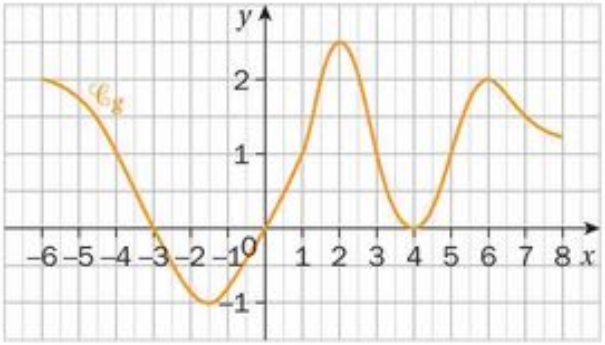
\includegraphics[width=10cm]{evaluation_16_graphique.png}
\end{center}

Résoudre graphiquement les équations et inéquations suivantes :
\smallskip
\begin{multicols}{4}
  \begin{enumerate}
    \item $g(x)=0$
    \item $g(x)=3$
    \item $g(x)>1$
    \item $g(x)\geq 0$
  \end{enumerate}
\end{multicols}

\dotfill\rep{8}

\bigskip

\exo[2 points] \vspace{-2mm}
\begin{enumerate}
  \item Inventer une inéquation faisant intervenir la fonction inverse et dont l'ensemble des solutions est \\$]-\infty;0[\cup]2;+\infty[$.\rep{4}
  \item Inventer une inéquation faisant intervenir la fonction racine carrée et dont l'ensemble des solutions est $[0;25]$.\rep{4}
\end{enumerate}

\end{document}

%%% Local Variables:
%%% mode: latex
%%% TeX-master: t
%%% End:
